\documentclass[12pt]{article}
\usepackage{graphicx} %required for inserting images
\graphicspath{{./images/}}
\usepackage{array}
\usepackage{lipsum}
\usepackage{comment}
\usepackage{amsmath}
%flowchart drawing package




%Tiles making sections
\title{GEOTECHNICAL DESIGN OF DRIVEN PILES UNDER AXIAL LOADS}
\author{Sakib Bin Rafi Tonmoy,Jakaria Pervez}
\date{05/04/2023}
%End for tiltles
\begin{document}
\maketitle

%%Begining of Introduction
\section{Settlement of Piled-Raft System with floating piles }
 Instllation process of Rammed Aggregate Piles can be thought of combination of bored and driven piles.Usual boring are made and soft soil are kept in place by using metal casings.Matreial for this type of pile shall be 70% coarse agrregate.Gravels are prefeable for cost minimization khoa may be used.Reamiander 30% is sand at top lift.This two lift are rammed using 15 to 20KN rammer dropped from 1.0m to 2.0m . \\
 
 
 %%adding figure for equivalent pier
\begin{figure}
\centering
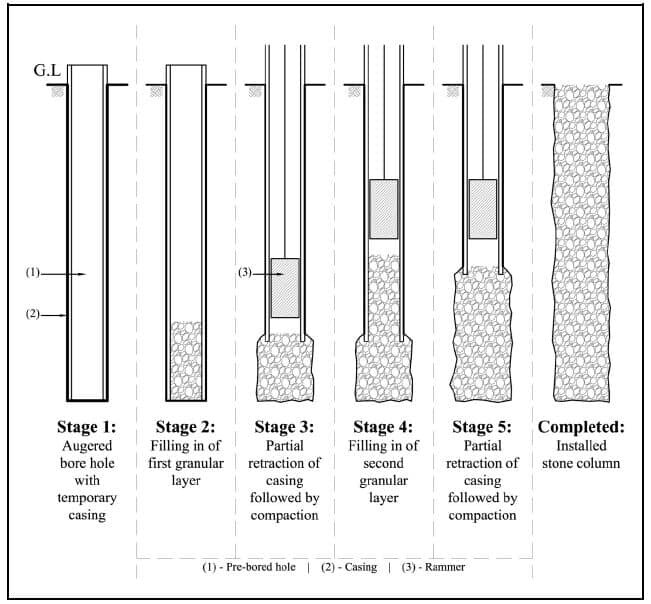
\includegraphics{stone-column-installation}
\caption{Rammed Aggrgate Column Instllation}
\label{fig:rammed_aggregate_column}
\end{figure}

%%end of figure






\begin{comment}

\begin{center}
\begin{table}
\begin{tabular}{|m{10cm}|m{2cm}|m{4cm}|}
\hline

                   & Limiting f,kips/fit^2(kPa) \\
\hline
Very loose & 15 & 1.0 (47.8)\\
\hline
Loose & 20 & 1.4 (67.0)\\
\hline
Medium & 25 & 1.7 (83.1)\\
\hline
Dense & 30 & 2.0 (95.5)\\
\hline
\end{tabular}
\caption{\label{f_non_cohesive}uideline for Side Friction in Siliceous Soil}
\end{table}

\end{center}

\end{comment}
\end{document}